\chapter{Architecture}
\label{chap:architecture}

The following section will define the data model each peer keeps of its data and specify the API for updating it between peers.
First we will define and explain the model each peer keeps of the stored data.
Next the messages used to facilitate the update of the model between clients will be discussed.
Finally we will take a look at the advanced features and how they will be built on top of the previous work.

\section{Peer Data Model}
\label{sec:Peer Data Model}

% why again json
Since we intend to use JSON for communication via Tox, it seems prudent to define the file model of a peer's data in the same way.
This will allow easy application of updates without having to explicitly translate between two different views of the same data.

An important feature that the model must have is that it works independent of the file types.
Therefore there are only two assumptions we will make of the structure of the directory that a peer will work on: namely that it contains files sorted in directories.
Out of this tree view we can immediately synthesize our two main components we will require: a file model (a leaf) and a directory model (a node).
Since a peer is intended to have directory as the root node from which to run, the core element will always be a directory.
An example of the proposed model structure can be seen in~\ref{list:model}.

\begin{figure}[htp]
\begin{modellist}
\item Root Directory
    \begin{modellist}
        \item .tinzenite Directory
            \begin{modellist}
                \item ...
            \end{modellist}
        \item Sub Directory
            \begin{modellist}
                \item File
                \item File
            \end{modellist}
        \item File
        \item File
    \end{modellist}
\end{modellist}
\caption[Data Model Example Structure]{An example of how a data model of a directory is structured. The .tinzenite directory is discussed in section~\ref{sec:Meta Data}.}
\label{list:model}
\end{figure}

The most important aspect is of course what information is stored within the model and its objects.
Each file is considered a binary blob and not modified by Tinzenite in any way to preserve data integrity.
Therefore additional information that Tinzenite requires to function will need to be part of the model.

Each object in the model will for identification purposes be specified by a hash.
This hash will be a unique randomly generated hash.
This hash allows us to decouple the name of the object from its model representation, effectively serving the same function as node identification numbers when stored on a disk.
This is required so that we can differentiate a renamed file from a removed file and update the model accordingly.
Furthermore each model object will contain a path variable that specifies the complete path of the object in the directory tree.
This has the purpose of allowing the placement of all files in the correct locations on disk.
Notably, unlike on the user's disk, the names contained in the path are the identifying hashes.

Apart from the above attributes Tinzenite must also track versions of files to allow detection of when files have been updated.
We will use a vector clock~\cite{mattern1989virtual} to implement this.
The vector of peers with the associated versions can also be used to detect collisions.
We avoid using a simple dirty flag for reasons of complexity: determining which peer's update to take in which order is not trivially doable with a simple boolean flag.

It is important to note that the model will not be used to store peer reliant information.
This includes for example where the directory is placed on the peer's file system.
Such information must be stored separately by the peer and applied when working with the data model, for example when determining what the full path on the file system will be for a file that is to be written.
Some properties are also not suited to be transferred between peers.
This includes file system or operating system dependent properties such as usage rights, ownership, or flags.

\subsection{Directory Model}
\label{sec:dir_model}

\begin{figure}[htp]
    \begin{lstlisting}[language=json,firstnumber=0]
    {
        "identification":"subdir_random_hash",
        "path":"root_hash/subdir_random_hash",
        "name":"subdir",
        "shadow":"false",
        "version":{
            "peer_name", "version",
            "peer_name", "version",
            ...
        },
        "objects":[
            ...
        ]
    }
    \end{lstlisting}
\caption[Directory JSON Model]{An example of a directory JSON object. Note that for brevity no files or sub directories are shown in the \textit{"objects"} array.}
\label{json:directory_model}
\end{figure}

Figure~\ref{json:directory_model} shows an example of the proposed JSON structure for representing a directory.
A directory is somewhat special as it does not require the synchronization of an attached binary file.
This is the case for Tinzenite because directories are viewed independent from their content in most cases.

The \textit{"identification"} attribute is a random generated hash that uniquely identifies the directory.
The \textit{"path"} attribute stores the concatenated relative full path from the peers root directory, notably replacing the real names of the directories with the corresponding identification attribute values.
For trusted peers that store an unencrypted version of the directory the clear text \textit{"name"} is also stored here as an attribute.
If the peer is encrypted the clear text is replaced by the encrypted version of it.
The \textit{"shadow"} flag is used to signal whether the contents of the directory are to be fetched or not.
Note that this flag is not indicative of whether any nested objects are also shadow objects\footnote{This means that the flag is only read on receiving update messages: if no different policy for the updated object has been set the directory flag is used to determine whether to fetch the actual file or not. Directories are always created on the file system though.}.
To differentiate between updates we require a \textit{"version"} attribute which represents a vector clock of peers and their last known version.
Finally an \textit{"objects"} array is where the corresponding sub directories or files are recursively placed.

\subsection{File Model}
\label{sec:file_model}

\begin{figure}[htp]
    \begin{lstlisting}[language=json,firstnumber=0]
    {
        "identification":"file_random_hash",
        "path":"root_hash/subdir_random_hash/file_random_hash",
        "name":"file",
        "version":{
            "peer_name", "version",
            "peer_name", "version",
            ...
        },
        "content":"content_hash",
        "shadow":"false"
    }
    \end{lstlisting}
\caption[File JSON Model]{An example of a file JSON object.}
\label{json:file_model}
\end{figure}

Figure~\ref{json:file_model} shows an example of the proposed JSON structure for representing a file object.
The \textit{"identification"} attribute is a random generated hash that uniquely identifies the file.
The \textit{"path"} attribute stores the concatenated relative full path from the peers root directory, notably replacing the real names of the directories with the corresponding identification hashes, and finally the file name with its hash too.
For trusted peers that store an unencrypted version of the file the clear text \textit{"name"} is also stored here as an attribute.
If the peer is encrypted the clear text is replaced by the encrypted version of it.
To differentiate between updates we require a \textit{"version"} attribute which represents a vector clock of peers and their last known version of this file.
Important for detecting file changes is the \textit{"content"} attribute which stores a hash of the file's binary blob.
Finally the \textit{"shadow"} flag is used to notify a peer whether the file is locally accessible or must first be fetched from other peers.
On sending updates it is also indicative to the receiving peer whether the file can be fetched from the sending peer: if the value is true than the peer does not have a copy of the file, only its object model (see also section~\ref{sub:Shadow Files}).

\section{Core Update API}
\label{sec:Core Update API}

This section describes the application interface that will be used to synchronize two models on separate peers where the models might diverge.
To understand how this works, it is important to understand how Tinzenite is structured.

Every peer views all connected peers as separate connections.
A swarm behavior only comes to pass because of the independent actions of every peer, not through a combined communication between multiple peers.
This primarily makes it relatively easy to implement a Tinzenite peer, as the communication state is never between multiple peers.
Therefore a single peer has a base state of no connected other peers.

\subsection{Connection Management}
\label{sec:conn_management}

In this section we will discuss how Tinzenite connects to other peers.
As we distinguish between trusted and encrypted peers we must determine how the data we will send is to be modified accordingly.
If the initiating peer is already encrypted, the connection by default will be considered anonymous.
If not the peer must query the other peer.
Since we can not trust the other peer to give an honest answer this query must be cryptographically secure.
Attackers that illegitimately wants to connect to a trusted peer thus can not establish a clear connection without the required keys, which they should not be in possession of\footnote{Tinzenite is designed to avoid revealing keys to outsiders. However outside attacks are beyond its control such as for example key loggers.}.
Only if the challenge is successfully replied to is the other peer considered trusted and the following communication not anonymous.
If the challenge is ignored the other peer is considered as an encrypted peer and the following communication adapted to fit.
Should the challenge be incorrectly answered we can consider possibly warning the user or even blacklisting the peer.

Once the connection type has been determined it will be applied to all following communication.
In general this means that compared to a trusted communication identifying information and file contents will be encrypted.
The peer list will be synchronized but the encryption keys not.
The model exchange and all update messages will be partially encrypted too to preserve data security.

The next and final step to a ready and idle connection state is the exchange of models.
Once this is done both peers can compare the received models with their local ones and determine which files they need to update from the other peer.
These messages will then be sent asynchronously over the now established and typified communication channel accordingly.

\begin{figure}[htp]
\centering
    \includegraphics[width=\textwidth]{graph/sm_peer_communications}
\caption[Connection State Diagram]{This diagram shows how peers handle the establishment of a connection to a known peer.}
\label{graph:connection_states}
\end{figure}

Figure~\ref{graph:connection_states} shows an informal state diagram of how a peer reaches the idle state where the connection is ready and set up.
The switch from the disconnected state to the connected state is signaled by the underlying Tox connection, meaning it happens when the other peer is online and visible via the Tox channel.
Once connected and if the peer itself is a trusted peer, a challenge is sent which contains a general identifier and an encrypted nonce.
The encrypted nonce is important to check whether the other peer is encrypted or trusted.

Note that a few points must be considered that can not be shown in the diagram.
Since Tinzenite is designed as a peer to peer network, no client server structure exists.
This poses the challenge of who begins the construction of a connection, especially as we can not distinguish between peers that have been online for a while already and peers that just activated when the base peer starts up.
This is due to peer to peer architecture of Tox: not all peers will respond to queries within the same time frame.
Peers further away from a network perspective will seem to be online only after peers that are nearer.
We solve this issue by having the peers use a random back off time whenever a request expects an answer\footnote{For example the challenge message for establishing a trusted connection.}.

Since we can not trust the other side of the Tox channel to be a Tinzenite peer, the peer initiating a connection will not advance beyond a step where it expects an answer.
This means that for example an attacker would either receive only a challenge (to which he can't respond without knowing the keys) or the anonymized model and peer list\footnote{The peer list is the more problematic of the two as it can be used to determine the size of the user's Tinzenite peer network. However to allow encrypted peers to facilitate file transfer between two mutually exclusively online peers, it must know this information. This is mitigated by the fact that Tox IDs are hard to guess and not shared beyond the Tinzenite peer network. TODO: move this to the security section / chapter / whatever?} (which doesn't offer up any useful information as per specifications).

\subsection{New Connection Establishment}

The previous section described how Tinzenite connects to known peers.
This section therefore discusses how Tinzenite connects to new peers, meaning peers that the user adds to the network.
Notably this is a manual process where the user is used as a secondary channel to prevent man in the middle attacks.
Since a typical Tinzenite network might have many peers, it is not desirable to have to authenticate a new peer manually with every other peer.
We therefore propose that the user only need authenticate the new peer with one existing peer.
From there the authentication is synchronized to the other existing peers much like any other file or property update.
This bootstrapping process allows a user friendly setup of peers.
Should the same peer have been added multiple times at different existing peers Tinzenite will detect this and merge the authentication together.

\begin{figure}[htp]
\centering
    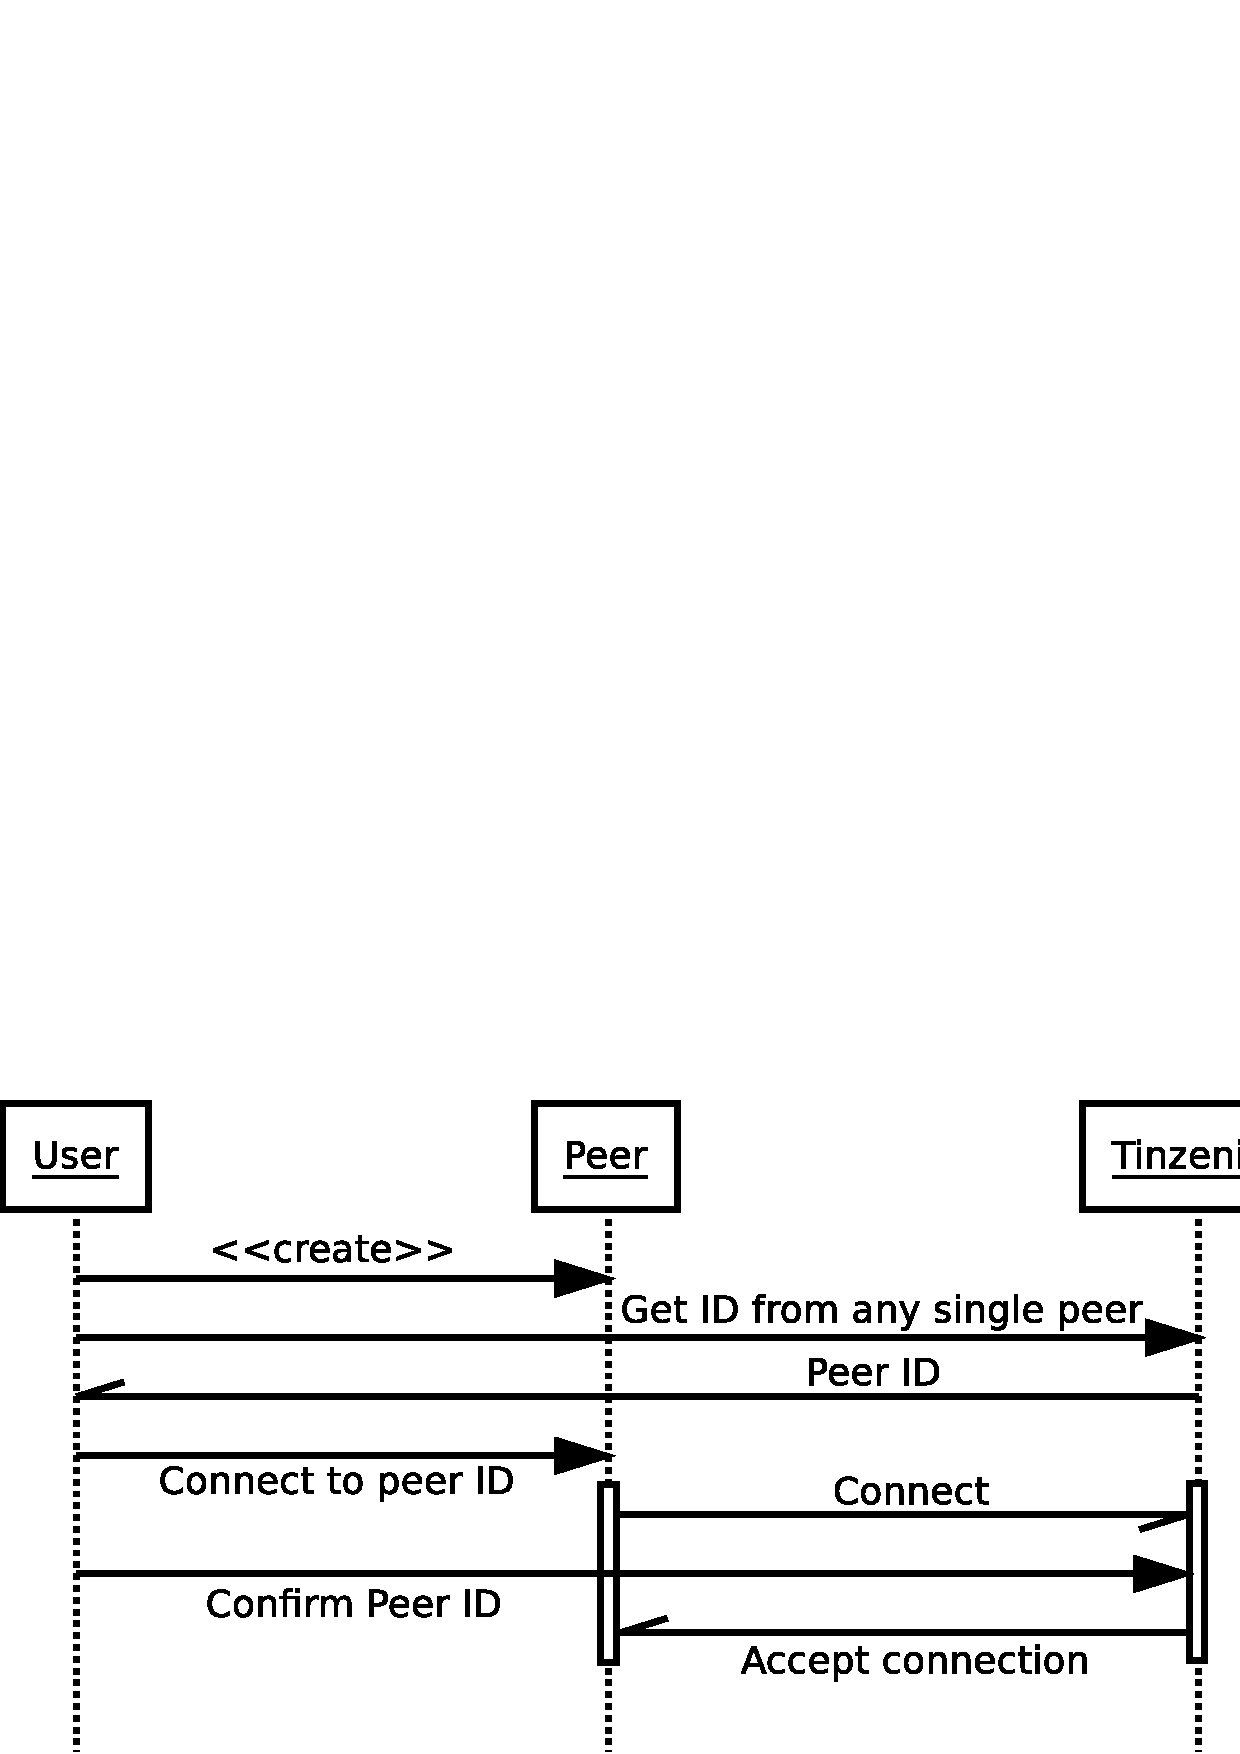
\includegraphics[width=10cm]{diagram/sequence_new_connect}
\caption[New Connection Sequence Diagram]{This diagram shows the interaction required to connect a new peer to the existing Tinzenite network.}
\label{diagram:new_connection}
\end{figure}

Figure~\ref{diagram:new_connection} shows how a user interacts with a Tinzenite peer and the Tinzenite network (consisting of 1 to n other existing peers) to connect a new peer to the network for the first time.
As prose: the users simply start the new peer client for the first time.
Then they can point it at the directory location, change settings, and check that another peer is visible.
To establish an initial connection a Tox ID of an available Tinzenite peer is required.
The users can then command the new peer to connect to this available peer by entering the Tox ID.
To ensure that no man in the middle attack can happen the users will now have to confirm the connection on the available peer.
This means allowing the connection there and ideally ensuring that the seen Tox ID is identical with the new peer's Tox ID.
Once the connection has been confirmed on the other peer a channel is opened.

The peer then receives the authentication block to set up the basic information it requires.
Notably this also allows the user to define the new peer as a trusted peer by entering the password that unlocks the encryption key used for the stored data.
Access to the key also allows the peer to respond to other peers as a trusted peer.
The new peer address and its information will now be synchronized throughout the already connected peers once they are available, removing the need to add the new peer manually to each and every one.

Now the channel has been established and the peers can begin communicating as shown in figure~\ref{graph:connection_states}.
Notably though the starting state is the \textit{"Connected"} state as the connection has already been established on the Tox layer.
Depending on whether the user has specified the new peer as a trusted peer by entering the password or as an encrypted peer by skipping that step the peer will be defined accordingly.
The directories will begin synchronization once the challenge and model exchange have happened.

Removing peers will work much in the same way from a system perspective.
A user can note a peer to be removed, resulting in it being removed immediately from the peer where the action was initiated.
It will then transit through online peers and result in a complete removal once all peers have been online.
An interesting aspect to how to handle removal from the perspective of the to be removed peer is what to do with the data on the peer.
For a trusted peer we might offer a choice whether to remove the data or simply disconnect it from the Tinzenite network.
On the other hand encrypted peers can simply remove the data immediately as they can't access it anyway.

\subsection{Model Management}

This section will describe how a peer receives and sends messages via the Tox channel.
Since we will be required to distinguish between encrypted and trusted connections we will start off with the trusted one and then briefly highlight the differences required for an encrypted connection.

Once the setup has been completed, as seen in section~\ref{sec:conn_management}, the models must be updated if they do not match.
This happens normally when files and directories have changed through user or system interaction.

\subsubsection{Fetch File Message}

\begin{figure}[htp]
    \begin{lstlisting}[language=json,firstnumber=0]
    {
        "operation":"fetch",
        "identification":"object_identification_hash",
        "TODO":"ADD LIBRSYNC STUFF HERE",
        "delta":"true/false"
    }
    \end{lstlisting}
\caption[Fetch Object Message]{The message sent to initiate a file transfer.}
\label{json:fetch_file}
\end{figure}

Figure~\ref{json:fetch_file} shows how a message to initiate a file transfer is structured.
Note that apart from the identification we require no further information – the model has been independently updated.
Now the peers need only get the binary files.
Upon receiving the message the other peer starts a Tox file transfer which the initiating peer knows to accept as it just requested it.

\subsubsection{Update Object Message}
\label{subs:Update Object Message}

\begin{figure}[htp]
    \begin{lstlisting}[language=json,firstnumber=0]
    {
        "operation":"create",
        "object":{
            ...
        }
    }
    \end{lstlisting}
\caption[Update Object Message]{The message broadcast by a peer to connected peers to notify that an update has happened. Operation can be any value of either create, remove, or modify.}
\label{json:update_object}
\end{figure}

Figure~\ref{json:update_object} is a message for broadcasting a model update to other connected peers.
The update message serves to keep both models in sync even after the initial synchronization at connection establishment.
Upon receiving an update message the peer will most likely immediately respond with a fetch message to retrieve the updated file.
If a peer receives a message for an operation that it has already applied, the message is silently discarded.
This does not disturb the propagation of updates since the peer will have already sent the update to the other connected peers if it has the update already.
In this way we ensure that every message propagates as far as possible without consuming unnecessary bandwidth\footnote{Peers are of course free to implement message sending in any way since the update messages are not critical for Tinzenite to work. Peers can simply only send update messages to a limited number of peers, down to none if bandwidth is scarce for example in the case of a mobile device.}.

\section{Object Operations}
\label{sec:Object Operations}

In this section we will discuss the object operations that Tinzenite requires to work.
Then we will specify the actual architecture of the messages we require for them.

TODO: allow and include a move update?
May well make a lot a whole bit easier to implement.

\subsection{Operations}
\label{sub:Operations}

Tinzenite relies on the most basic file operations for manipulating both the model and the actual file directory.
Therefore we require only the following three operations for the basic case to work:

\begin{description}[leftmargin=5em,style=nextline,noitemsep,nolistsep]
    \item[Create]
        Files that have been created will be added to the model at the correct location and their attributes calculated, if not given.
        Tinzenite then checks whether it needs to fetch the file if it wasn't created in its own directory.
        Created files are detected by simply noticing files that do not exist in the model yet and are not listed as deleted.
    \item[Remove]
        File removing is one of the most complex cases in Tinzenite due to the insert delete ambiguity (see section~\ref{sub:Perspectives on Optimistically Replicated, Peer-to-Peer Filing}).
        We solve this by storing the models of deleted files until the delete update has propagated to all currently known peers.
        Only then is the model discarded also.
        For this to work Tinzenite must always ensure that files that exist but are listed as deleted are not added back to the model as a new file by continuously checking the deletion list.
    \item[Modify]
        Modification is either when the model does not match the file anymore, in which case a new file must be fetched, or the content on the local file has changed.
        This is detected via the content hash.
        In that case the model is updated to match the file again.
\end{description}

Of course those three operations are not the only operations that a user can do on directories or files.
However they are all the operations that Tinzenite requires so that it can offer full functionality.

Renaming objects can be handled by simply considering the old file to have been deleted and replacing it with the new file.
This new file will just so happen to share the same content hash.
Moving objects are handled much in the same way: by removing the file at its old location and creating it anew at the new location.
Peers are of course free to go about removing and moving files in a more intelligent manner, saving the costs of fetching a renamed or moved file from another peer if the data is already locally available.

\begin{figure}[htp]
\centering
    \includegraphics[width=4cm]{graph/sm_object_lifecycle}
\caption[Object State Diagram]{The life cycle of every object, file and directory, in Tinzenite with the allowed operations.}
\label{diagram:object_operations}
\end{figure}

Therefore the life cycle of an object is very simple, as can be seen in figure~\ref{diagram:object_operations}.
Objects can only come into existence via the create operation.
Once an object it is only possible to either modify the existing object or remove it.
If an object has been removed it will stay removed unless the user creates a new clone of it.

\subsection{Specifications}
\label{sub:Specifications}

In this section we show the actual definition of the specification and expand on how Tinzenite peers react to them in detail.
This specification makes up the core functionality of how the data synchronization happens within Tinzenite.
Note that only trusted peers can initiate object operations: encrypted peers only react to messages and propagate them, never do messages originate from an encrypted peer.
This is simply the case due to the fact that encrypted peers store the data in a non accessible format, therefore making operating on the data rather pointless.

\subsubsection{Create}
\label{subs:Create}

The creation of an object can be trivially detected in Tinzenite.
Basically there are two cases where an object must be created: the first is local manual creation which implies that the peer is the origin of the file; the second is creation via receiving an creation message from another peer.

For the first case, if the object does not have a representation within the model and is not listed as deleted, it triggers the creation case.
Tinzenite creates the correct object representation and inserts it into the correct place in the model.
In the second case the peer will queue a fetch operation for the required file\footnote{Note that in the case that it receives an update with a set \textit{"shadow"} flag it will not try fetching the file from said peer as it doesn't have a copy of the file. As a special case files within shadowed directories will also never be fetched.}.
Only when the file has been received completely is it placed at the correct location and the model updated.

After the local model has been updated and everything is in order, the peer will send an update message to all connected peers.
Figure~\ref{json:update_object} shows how such a message might look – note that the operation is labeled as \textit{"create"} accordingly.
It is then up to all receiving peers to update their models and fetch the file, then propagate the update accordingly.

\subsubsection{Modify}
\label{subs:Modify}

The modification of an object is not as trivially detected as an object creation – for the specifics of update detection see the following section~\ref{sec:Update Detection and Reconciliation}.
Here we will only concern ourself with what happens once a modification has been detected.
Again we have two cases for triggering this case: a local file has been modified or the peer has received an update message.

If the modification is detected locally first we update the model to match and then initiate an update message.
The message is of the format as shown in figure~\ref{json:update_object} with the operation now reading \textit{"modify"} instead.
If, on the other hand, we receive such a message, we queue the fetching of the updated file.
Upon receiving the changes we apply them and finally propagate the update to the other connected peers.

\subsubsection{Remove}
\label{subs:Remove}

Finally the deletion of an object is the hardest case within Tinzenite because of the insert delete ambiguity as discussed in section~\ref{sub:Perspectives on Optimistically Replicated, Peer-to-Peer Filing}.
It is non trivial to ensure that an object deletion has been received by all required peers so that it truly and finally can be removed from the system.
A simple solution would be a list of all ever deleted objects, but unlike removed peers this list promises to grow quickly on often used synchronized directories.
Therefore we require a sort of garbage collection so that we can trim the list from deleted files that have been applied to all known peers.

For the base case we will look at how Tinzenite deletes an object that has been removed locally first, then discuss how the update propagates and what the other peers are required to do to ensure a safe and complete deletion.
If a deletion happens the object and object model are moved to a special directory outside of the user viewable directory (see also section~\ref{sec:Meta Data}).
Then the peer copies the list of currently known peers and places it with the object model.
Finally it creates a second list of peers in which it places itself.
This second list contains all the peers that have acknowledged receiving the deletion update.

This deletion update is then propagated to the other peers.
Each peer receives the update, moves the object and updates the object model, enters itself into the second list, and propagates the update.
Once the last peer enters itself into the acknowledgement list, thus making it equal to the first list of peers, it propagates the update one final time and can then delete the object model from the deletion space and the actual object.
The completed deletion update then traverses the peers backwards, each in turn deleting the update from its list and propagating it a last time.
Thus when the last peer to receive the full deletion update removes the model, we can be assured that all relevant peers have removed the object.

It is not immediately obvious why this works even should new peers be created while the deletion update is in progress.
In fact this is only possible by adding a small modification to the outlined process.
To show that the solution can work with the small modification we need to look at the two cases that can happen for a newly created peer, differentiated by where it first connects to.
If it connects to a peer that has already received the deletion update the solution would work by default without any modification.
This is the case since the new peer would receive the object model where the object has already been deleted.
It must thus not be notified of the deletion.
If, however, it connects to a peer that has yet to receive the deletion update even though it has already happened, we have a problem.
The new peer is not listed among the peers that must acknowledge the update even though it has the object.
Without the modification, this could result in the file being reintroduced by the new peer, undoing the deletion in effect.

Therefore peers must expand the first list of known peers if a single criteria is met.
This criteria is relatively straightforward: when receiving a deletion update each peer first checks the list against its own known peer list and in the case that they differ add all missing entries to the deletion update.
If a newly created peer has connected it will already be within the list and thus be ensured to have the deletion update hang around until it has received it.

Now a final note on what happens should a peer receive a deletion update for an object that it doesn't know.
In this case the message can not simply be silently discarded as there is no other representation of the update in the object model.
This could lead to orphaned updates if the peer acts as a bridge between two peers that were previously directly connected.
Therefore unknown deletion updates should be propagated if possible.
However, since orphaned updates can only happen as long as the peer list has not been fully updated between all peers, this is a sufficiently unlikely case that we can live with it.
By adding a time stamp we can even detect orphaned deletion updates and warn the user to help in solving the issue.
Alternatively we can also warn if we have too many possibly orphaned updates, although this would signify a larger issue.

\section{Update Detection and Reconciliation}
\label{sec:Update Detection and Reconciliation}

This section describes the theoretical side of the update detection: how we detect updates on file systems in a way that does not consume too much resources of the hosting computer.
Then we will discuss the interesting case of update reconciliation and how Tinzenite reacts to conflicts.

\subsection{Update Detection}
\label{sub:Update Detection}

Tinzenite continuously checks the directory against the model of the same (see also TODO).

%TODO
TODO write.
Directories MUST always check sub directories for changes before you can delete or modify them (at creation time they are empty by default).
Can directories only be removed if all sub files are removed first?
This could be a sensible way to implement this...

TODO.
I'm not sure how I can implement this yet and whether I will use an external library for a file watcher.
I'll get back to this at a later point in time.

\subsection{Update Reconciliation}
\label{sub:Update Reconciliation}

The core algorithm for how update reconciliation is done is another important element of Tinzenite.
The following section introduces it and discusses the ramifications for the system based on the initial model synchronization, leaving aside the per object update messages at first.
These will be discussed once the basic mode is understood.

The reconciliation begins by receiving the model of the other peer.
The model is temporarily stored so that Tinzenite can work with it until the reconciliation has finished.
To guarantee that the directory remains consistent with the model right from the start we propose a simple rule: the model of the local directory is updated atomically with the successful reception of the binary object updates.

For each object in the received and temporarily stored model Tinzenite performs a series of checks.
For the sake of decreasing algorithm complexity we start with the easy case of file creation.
In this case the object has not previously been stored in the local model.
This is the case when a file has been newly created on a remote peer.
We can thus request the object from the remote peer without further logic required.

If the object is listed in the deleted list we can possibly ignore it outright.
This would mean that the other peer has not received the deletion message yet.
To avoid reintroducing already deleted objects they thus have to be ignored when reconciling.
If however the objected has been modified we must reconcile this conflict.

If the object has neither been deleted nor created it can only have been modified.
As this is where conflicts can regularly happen the case is somewhat more complex.
There are two simple paths here: if no modifications have happened either remotely or locally, nothing further must be done.
If changes have been made remotely but not locally we can simply request the updated object from the remote peer and are also done.
If, however, we detect both local changes that the remote peer does not know of and remote changes that are new to us we have found a conflict.

Tinzenite uses only the model objects to detect changes, specifically only the version attribute.
As shown in section~\ref{sec:Peer Data Model} the version attribute contains a list of peers and the last known version of the object they have.
From this list we only ever are interested in the versions of the remote peer and the local peer.
By comparing these two attributes between the versions that both peers have we can reliably detect how to proceed without losing data.

\begin{table}[htp]
\centering
\begin{tabulary}{\textwidth}{J || J | J }
      & Local object not modified & Local object modified \\
    \hline \hline
    Remote object not modified & Nothing & Nothing (It is up to the remote peer to actively fetch this update.) \\
    \hline
    Remote object modified & Fetch remote object and apply update & Resolve conflict \\
\end{tabulary}
\caption[Peer Object Version States]{This table shows the four possible cases that can result from comparing the versions between two peers.}
\label{table:version_states_possible}
\end{table}

Figure~\ref{table:version_states_possible} shows the four possible cases.
Since there is nothing to do independent of our local state if the remote peer has no modifications, Tinzenite will check this first.
This is done comparing the locally last known version of the object from the remote peer with the version the remote peer how has of the object from the temporarily stored model.
If it is equal we can continue on to the next object.

In the case that the remote object has a higher version number since the last synchronization we check first whether changes have been made to the local object.
If not we can simply request the new version of the object and apply it to our model.
However if we detect that our local object has also been updated we have ourselves a conflict.
How this conflict is resolved is discussed in the next section.

\subsubsection{Conflict Reconciliation}
\label{subs:Conflict Reconciliation}

As stated before Tinzenite considers files to be atomic entities and thus will not modify them itself.
Therefore no automatic conflict resolution will be implemented in the base Tinzenite system.
Thus Tinzenite must support the user in resolving conflicts.
We do this by clearly labeling conflicts by appending a special word to the object name, possibly also referencing which operation has happened (either create, modify, or remove).
So now we must store both versions of the conflict in a way that it can be easily resolved on any peer.

The solution we propose is in itself simple enough from a technical view.
Basically, we remove the old version of the object and replace it with the two conflicting versions.
As these are newly created files they can propagate through the network as any other object would, allowing the conflict resolution to happen even on peers that did not see the conflict initially.
It is then up to the user to either keep both versions (likely renaming them) or merge the changes into one object and removing the other.
Both cases will be propagated through the network as normal file operations.

So for an extreme example case consider the following: a file present on two peers is modified on one peer but deleted on another.
Now they synchronize and detect the conflict.
Since by definition the deletion can not already have fully propagated as the other peer still could modify the object the file is still present in the meta data directory (see section~\ref{sec:Meta Data}).
Therefore both peers can access the other's version of the object and reintroduce it in the user viewable directory as normal conflicting updates.
The deletion update will be overwritten by the higher version update of moving the file to its conflicting state, thus ensuring that it will not remain valid for long.

\section{Meta Data}
\label{sec:Meta Data}

Special files and temporary storage space is offered by a hidden directory directly below the root directory.
It will be specified as \textit{".tinzenite"} in a comparable manner to the \textit{.git} directory for Git.
In short it contains organizational files, temporary objects, and the deletion directory for storing files until they have been fully removed by all peers.
Figure~\ref{list:meta_folder} gives a broad overview of the proposed contents.

\begin{figure}[htp]
\begin{modellist}
\item .tinzenite
\begin{modellist}
    \item .tinignore
    \item org
    \begin{modellist}
        \item auth.json
        \item peers
        \begin{modellist}
            \item peer.json
            \item ...
        \end{modellist}
    \end{modellist}
    \item removed
    \begin{modellist}
        \item ...
    \end{modellist}
    \item temp
    \begin{modellist}
        \item ...
    \end{modellist}
\end{modellist}
\end{modellist}
\caption[Meta Folder Structure]{Overview of the special meta information directory that Tinzenite uses to store relevant information required for the managing of the directory.}
\label{list:meta_folder}
\end{figure}

Placing the meta data within the directory has a few benefits for the complexity of the system and enables it to utilize the full feature set of the implemented synchronization capabilities.
The directory is only special in how conflicts are handled as the user should never have to resolve conflicts of meta data manually.
We will therefore shortly note in each of the following sections how Tinzenite will handle the special cases if applicable.

\subsection{Organizational Directory}
\label{sub:Organizational Directory}

The \textit{"org"} directory consists of two objects: the file containing the authentication information and a sub folder which contains a file for each known peer.
Every file will be a simple text file with JSON contents.
Figure~\ref{json:auth_object} shows the contents of the authentication file.

\begin{figure}[htp]
    \begin{lstlisting}[language=json,firstnumber=0]
    {
        "user":"hash_of_username.salt",
        "directory_id":"random_hash",
        "key":"encrypted_data.salt"
    }
    \end{lstlisting}
\caption[Authentication JSON Object]{Shows the proposed contents of the authentication file.}
\label{json:auth_object}
\end{figure}

TODO: note that the peer objects include the user given peer name, required for conflicts.

\subsection{Removed Directory}
\label{sub:Removed Directory}

\subsection{Temporary Directory}
\label{sub:Temporary Directory}

TODO: note that the .tinignore file is for this folder as the contents are peer local.

\subsection{OLD}
\label{sub:OLD}

Partially fetched files are stored in a special non synchronized sub directory\footnote{TODO: this depends on how I receive the files from Tox. If I get the complete thing this is unnecessary. Would be an easier case because the meta dir would require an ignore file by default.}.
Another directory is used to store deleted files that have not yet propagated to all peers.

TODO: following is old stuff, merge into above.

Apart from the model of the directory for reconciliation each peer requires further information to work.
The following short section describes the further information that strictly speaking does not belong to the directory model, but is still required for Tinzenite to work correctly.
This information is stored within the hidden .tinzenite directory in a dedicated sub directory.

TODO: Below here everything needs to be adapted...
This block might be totally doable as files within the meta directory, thus easily allowing updates.
Proposal for this: make a sub dir in .tinzenite for it.
Place there one file that is the actual auth block and two folders for the two peer lists.
Each peer entry in the list is its own file within these folders.
Thus removing peers can easily be done and even later be added back again.
The implementation of white lists and black lists is thus easily doable too.

Figure~\ref{json:auth_object} shows the management block that a peer keeps.
The value of \textit{"user"} allows the allocation of a directory to a user name.
This is important for example for the support of encrypted third party peers: they can attach accounts to the provided user name for controlling server side access.
Therefore we also need a way to distinguish multiple synchronized directories from each other: this is the random unique hash stored in \textit{"directory\_id"}.
Again, this can be used by third party service providers to differentiate the amount of directories that a user can store with them.
The symmetric key for encrypting and decrypting data for encrypted peers is stored in \textit{"key"}, encrypted in turn by a to be defined scheme that decrypts it upon entry of the correct password by the user.

Note that changing any of the values in the authentication block is not supported initially beyond modifications of the peer lists.
To change the password or the user name hash, the Tinzenite peer must be removed and added anew.
While cumbersome it offers the highest level of protection against possible security risks for now.

Finally we also use the authentication block to store and synchronize the peer list of connected peers of a synchronized directory.
As peers can be removed we need to keep a list of removed peers too.
Peers that have been removed, thus placing their Tox identification within the removed list, can not be reactivated.
The peer must be recreated and added as if it were a new peer.
Since we do not expect a large number of peers to be removed and added over the lifetime of a Tinzenite directory, this list is never trimmed.
A peer can detect a new peer by noticing its existence upon synchronization with another peer.
If the new peer Tox identification is not in the removed list it is simply added to the active list.
This ensures that peers that have been removed will never be added back to the active list which might pose a security risk\footnote{TODO: do something similar for removing files. Note that we WILL have to trim that list though at some point in time, but since we know which peers are active, this should be doable.}.


\section{Advanced Features}
\label{sec:Advanced Features}

In this section we will describe the features that we consider to be advanced features.
These will for the most part be implemented at a later stage and are not relevant for the core functionality of the Tinzenite system.

\subsection{Space Management}
\label{sub:Space Management}

One feature that should be implemented is that peers can have a limited amount of available space without breaking the protocol.
This feature can be used to control how much data a mobile device has to synchronize at any given time or for the server peer, thus allowing control over how large directories maximally are.

Each peer is required to enforce the size restriction given by itself.
If the size limit has been reached it should only allow further updates as shadow files.
The interesting case is of course what happens to files that are modified above the limit: we propose either making the file a shadow file as soon as it crosses the limit or allowing modifications to push the size above the limit.
Since shadow files are already part of the Tinzenite protocol no further protocol support for this feature must be considered.
It is up to the server peer to implement this in a safe and user friendly way.

\subsection{Ignored Objects}
\label{sub:Ignored Objects}

To allow a user to only synchronize objects that they consider important another advanced feature we would like to implement is the ability to specify files and directories to be ignored.
An example for how we propose to implement this feature is the Git source control management software~\cite{web:site:git}.
By specifying the paths to directories and files within a so called \textit{.gitignore} visibility of these can be finely controlled.

In Tinzenite we plan to implement this functionality in a similar manner.
The file containing these rules can be synchronized just as any other file at any level within a directory.
Any new objects detected by Tinzenite that are listed in this file will not be created within the model, effectively keeping it out of the system.
Since it may well happen that such a file is created at a later point and thus introduce an uncertainty in handling the to be ignored files we propose a simple solution: the file is only ever applied for object creations.
Once a file has been created within the model it will be modified and deleted as any other file within the system, independent on the ignore file.

This in turn however means that renaming or moving a file in Tinzenite will remove it from the model, deleting it everywhere.
Since we believe this to be a feature for more advanced users we will not make this feature a core aspect of the system.
Normal users should have little need for only synchronizing a selected subset of files.

\subsection{Shadow Files}
\label{sub:Shadow Files}

Depending on the location of a client a user may with to only access specific files without having to get an entire set or updates.
This is a nice feature to have in the case of space and bandwidth restricted devices such as mobile devices.
By selecting specific files the client will then only update or retrieve the corresponding files or directories, ignoring the rest.
This works by fully synchronizing the model and creating placeholder empty files for every shadowed file.
By selecting a shadowed file it can be unshaded, resulting in Tinzenite trying to fetch the binary blob normally with all updates until it is again shadowed.

Functionality for the shadow file feature is available via the shadow attribute.
It affects only files directly as the creation of directories is not significant from a size point of view.
The attribute only serves as a shortcut to set all files of a directory implicitly to being shadowed.
If files are marked as shadow files they are not updated on the disk, only their model.
By setting the shadow flag to true the client will then immediately try to fetch the binary file from connected and available peers.

Of interest are then a few edge cases.
First and most trivial: what happens to an already synchronized file when the shadow attribute is set?
We propose that the file is immediately removed although this could be expensive in terms of bandwidth if the users quickly change their mind again as the file must then be fetched all anew.
A more sophisticated approach would integrate the size restriction capability of the client as proposed in section~\ref{sub:Space Management}.
By setting the space limit to a number below the full size of the directory files will only be immediately removed if near the space limit.
If the user changes their mind the file may thus still be immediately available.

So what do peers do if they receive a model update where the shadow flag is set?
It is important to note here that the shadow flag is considered to be transient when synchronizing models, meaning its value is considered to be local only.
However it is still sent as it is used to determine for the receiving peer whether it can fetch an update if applicable from the other peer.
Again it is up to the peer what happens upon receiving a shadow file update: trivially a peer that has a non shadow copy of the file will ignore shadow updates as it can not fetch the binary file update successfully from it.
It will then have to wait for another peer to offer the update where the attribute is not set.

The better solution would be to introduce a third value for the shadow attribute: temp.
This value is to be set when the peer knows of an update and has applied it to its model but has not fetched the binary file update yet.
When connecting to other peers the peer can then request all available files marked as temp and fully update them as required.
This approach has the added advantage of allowing a peer to notify the user that the file has been updated but not fetched yet.
We may also use this functionality to signal slow network transfer speeds: the user could at a glance see that the update is pending, possibly avoiding unnecessary conflicts.

The final edge case is an unpleasant one: what Tinzenite does not provide is a way to ensure that one full copy of the shadowed file is kept.
If the user marks a file as shadowed on all peers it may well happen that Tinzenite loses the file.
For now we propose to avoid this by explicitly warning the user of this possibility.
One way to mitigate this risk is by allowing user defined shadowed files only for specific clients: we can probably assume that any full desktop peer should always retain a full copy of the directory anyway.

%TODO: Is this a future work todo?

\subsection{Encrypted Peers}
\label{sub:Encrypted Peers}

The final advanced feature that is vital for the encrypted peer for third party support is how encryption is handled within the protocol.
Trigger for detecting that a peer is encrypted is when the challenge is not correctly responded or denied (if it outright fails Tinzenite probably should warn the user as it would mean that someone is trying to guess the response).
Once the other peer has been identified as an encrypted peer it is up to the local peer to enforce the correct encryption on files and obfuscation on model objects.

Every attribute that contains user information is encrypted with the encryption key.
Primarily within the model this means that the object \textit{"name"} is encrypted.
Apart from this attribute only the content hash is different although not encrypted – it is instead the hash of the encrypted file.
The file itself is fully encrypted when the peer receives a fetch request from the encrypted peer.
Only ever this encrypted file is to be shared.

In the base case each received fetch results in the complete requested file to be encrypted in its current version and sent.
Note that it well may be impossible to support sending only binary deltas of changes to an encrypted peer due to a single change within the file resulting in a completely new encrypted cipher representation of the file.
We will look into this again if we have the time to optimize the logic of clients.
We believe that by choosing a correct block cipher we can optimize this by sending only the changed blocks at the cost of some security.
